\chapter{Regression}

As with anything ML related, the Andrew NG course will help - and material from this was used to teach this topic.

In regression, we have a continuous range or set of labels that we try to predict. There are various degrees of functions that we can try using to model the data such as linear or quadratic.

Our features for a regression could be continuous, binary, or something else entirely too. Regression is primarily concerned with the range not the domain.

Input data could be weight and height of a person, making input a $R^2$ vector. \[ X = \{x^1, \cdots, x^n\} \text{ where } x^i \epsilon R^d \]

\section{Linear Regression}

A general linear regression hypothesis looks like:

\begin{equation}
    y \; = \; \theta_0 + \theta_1x_1 + \theta_2x_2 + \cdots + \theta_dx_d = \Sigma_{j=0}^{d} \; \theta_jx_j
\end{equation}

Hence, we have $d+1$ parameters to determine since the input has $d$ features and we have another constant (is like a bias).

The error is usually the L2 norm or sum of the squares of difference from the best fit line values. The cost function is:

\begin{equation}
    J(\theta) = \frac{1}{2n} \: \Sigma_{i=1}^{n} (h_{\theta} (x^{(i)} - y^{(i)})^2
\end{equation}

We need the cost function for the machine learning algorithm to optimize the accuracy of the model. The $\frac{1}{2n}$ part is purely to make the derivative easier to use. Here, $y$ is the correct function and $h$ is our hypothesis function for the set of parameters $\Theta$. We find the line of best fit for the parameters $\theta$ that minimize $J(\theta)$. We square the error since we do not care about the sign of the error - but rather the magnitude of the difference. 

The cost function for a linear regression is a convex function.

\subsection{Convex Function}

A convex function is such that between any two points $(x, f(x))$ and $(y, f(y))$, the values of the function in between all lie below these points. This is because:

\begin{equation}
    f(\theta x + (1-\theta)y) \leq \theta f(x) + (1-\theta)f(y) \text{ where $\alpha \epsilon [0, 1]$ }
\end{equation}

This part has been taken from \href{http://mathgotchas.blogspot.com/2011/10/why-is-error-function-minimized-in.html}{a nice blog}:

\subsubsection{First-order condition of convexity}

A function $f$ which is differentiable is convex if the following inequality condition holds true:

\begin{equation}
    f(y) \geq f(x) + \nabla_x^T f(x)(y-x) 
\end{equation}

Intuitively, this condition says that the tangent/first-order-taylor-series approximation of f(x) is globally an under-estimator.

\subsubsection{Second-order condition of convexity}

A function $f(x)$ which is twice-differentiable is convex if and only if its hessian matrix (matrix of second-order partial derivatives) is positive semi-definite, i.e.

\begin{equation}
    \forall z: z^T \nabla_x^2 f(x) \; z \geq 0 \text{ where } \nabla_x^2 f(x) \text{ is Hessian }
\end{equation}

\subsubsection{Linear Combination}

Let $f(x)$ and $g(x)$ be two convex functions. Then any linear combination of these two functions is also a convex function (this can be easily proved using the definition of convex function).

There's also an odd semester course - \textit{Applied Optimization (Prof Pawan Kumar)} where these concepts are covered in detail. Main reference is the book \textit{Convex Optimization by Stephen Boyd}.

There is no local minima or maxima for a convex function - there is just a global minima or global maxima. This can be proved easily using just the definition of the convex function. Most of the cost functions that we come accross won't be a convex function - and hence will have local minimas.

\begin{figure}[ht]
    \centering
    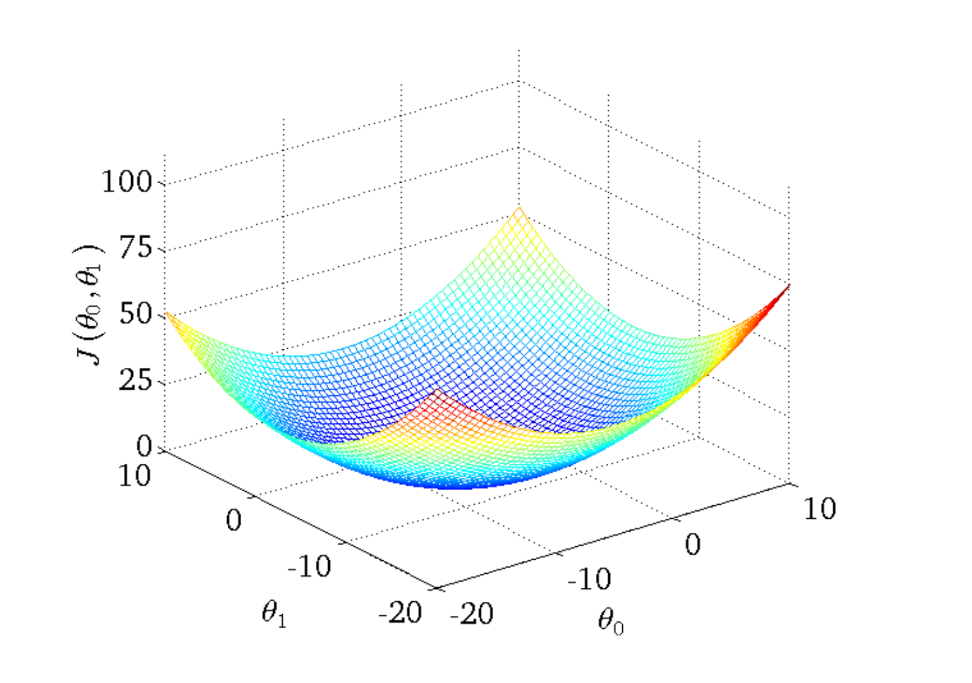
\includegraphics[width=9cm]{img/convex-cost-fn.png}
    \caption{Convex Function Depiction for Cost Function}
    \label{fig:cost-linear-regression}
\end{figure}

\section{Searching for Maxima/Minima}

For non-convex functions, we can have several local minimas and local maximas. Hence, we need a search procedure that can help us "climb up" or "climb down" a hill. Popular methods to do this include Gradient Descent and ADA

\begin{figure}[h]
    \centering
    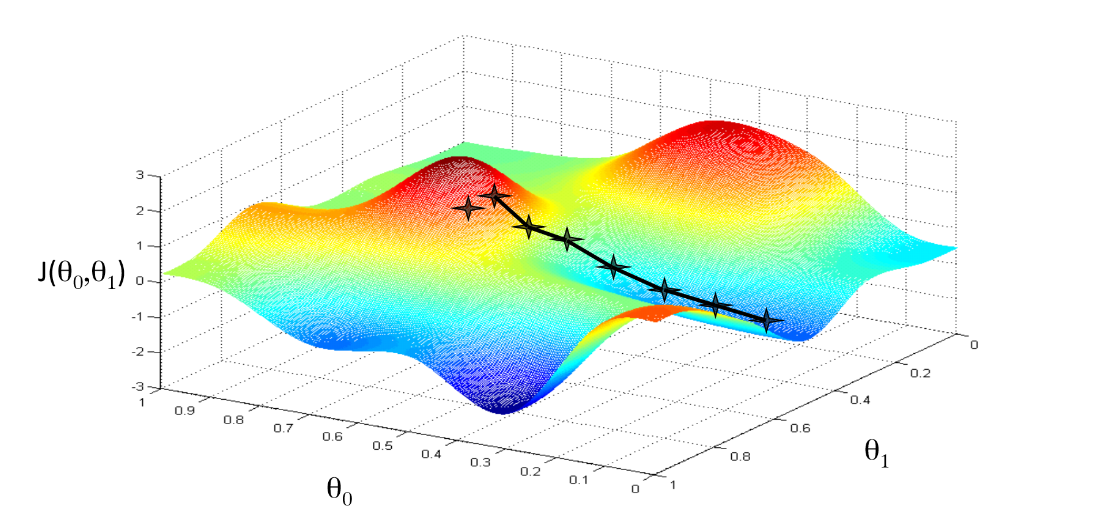
\includegraphics[width=9cm]{img/search-space.png}
    \caption{Search Space Example}
    \label{fig:search-space-example}
\end{figure}

\subsection{Gradient Descent}

The update function for gradient descent is:

\begin{equation}
    \theta_j = \theta_j - \alpha \frac{\partial}{\partial\theta_j} J(\theta)
\end{equation}

This update is done simultaneously to all parameters ($d$ of them). $\alpha$ refers to how quick/large our learning rate is. Essentially, we are moving at an $\alpha$ rate along the function. Larger the $\alpha$, the greater is the step taken.

\subsection{Cost Function Using Taylor Series}

We know that the cost function $J$ for weights $w$ can be defined as $J(w)$. Now, these weights weren't randomly created but rather the result of previous iterations. Or, 

\begin{equation*}
    w^{k+1} = w^k - \alpha\frac{\partial}{\partial w}J(w^k)
\end{equation*}

Now, for vectors, the partial derivative would infact be the gradient. Rewriting, we can say:

\begin{equation}
     w^{k+1} - w^k = -\alpha \nabla J(w^k)
\label{wk}
\end{equation}

Coming to the cost function once again, the cost function $J(w^{k+1})$ can be written as:

\begin{equation}
\begin{split}
    J(w^{k+1}) = J(w^k) + [w^{k+1} - w^k]^T\cdot \nabla J(w^k) + \frac{1}{2}[w^{k+1} - w^k]^T\nabla^2[w^{k+1} - w^k] + \cdots
\end{split}
\label{cost-fn-2}
\end{equation}

Here, we have used the Taylor series to write the cost function. To represent this purely in the form of its derivatives, we must rewrite $[w^{k+1} - w^k]$ in the form of equation \ref{wk}:

\begin{equation}
\begin{split}
    J(w^{k+1}) = J(w^k) + -\alpha \nabla J^T\cdot \nabla J(w^k) + \frac{1}{2}-\alpha \nabla J(w^k)^T\nabla^2J(-\alpha \nabla J(w^k)) + \cdots
\end{split}
\label{jcost}
\end{equation}

\subsection{Ideal Learning Rate}

We can set $\alpha$ depending on the iteration or the point it is at. There is a formula to choose the optimal value of $\alpha$ that uses the hessian. In general, we do not use the hessian since it is computationally intensive and fixing a small value of $\alpha$ will suffice. 

\begin{equation}
    \alpha = \frac{\norm{\nabla J}^2}{\nabla J(w^k)^TH[J]\nabla J(w^k)}
\end{equation}

The above equation can be derived as follows:

If we assume a second order approximation for cost function, we can represent the cost function as follows:

\begin{equation}
\begin{split}
    J(w^{k+1}) = J(w^k) - \alpha\nabla J^T\nabla J(w^k) + \alpha^2 \frac{1}{2} \nabla J(w^k)^TH[J]\nabla J(w^k)
\end{split}
\end{equation}

where $H[J]$ is the Hessian of the cost function (easier to use this notation). Now, to calculate optimum learning rate $\alpha$, we can consider the above equation to be a function of $\alpha$. On taking the derivative of the equation and equating to zero, we should be able to find the optimal value of $\alpha$!

\begin{equation*}
\begin{split}
    &\frac{\partial}{\partial \alpha}J(w^{k+1}) = 0 \\
    &\implies \frac{\partial}{\partial \alpha} (J(w^k) - \alpha\nabla J^T\nabla J(w^k) + \alpha^2 \frac{1}{2} \nabla J(w^k)^TH[J]\nabla J(w^k)) = 0 \\
    &\implies -\norm{\nabla J}^2 + \alpha \nabla J(w^k)^TH[J]\nabla J(w^k) = 0 \\
    &\implies \alpha = \frac{\norm{\nabla J}^2}{\nabla J(w^k)^TH[J]\nabla J(w^k)}
\end{split}
\end{equation*}


Unvectorized calculations of how the partial derivative is taken and calculated can be seen in slide 23 \href{https://github.com/RoboticsIIITH/summer-sessions-2020/blob/master/lecture-slides/deep_learning/linear_regression.pdf}{here}.

We repeat this update function \textbf{until convergence}. This essentially means - stop when the value tends to not vary much. In general, a popular converge is the L2 norm:

\begin{equation}
    \norm{\theta_{new} - \theta_{old}} < \epsilon
\end{equation}

We will notice that slowly and steadily, the global minima will be reached and the value of cost function will reduce, though at a slower rate as iteration count increases.

Coming back to the $\alpha$ value, if we set something too small, it will not converge soon (very slow), but if it is very large, we can actually \textit{diverge}. It may overshoot the minimum and even fail to converge. To see if gradient descent is working, print $J(\theta)$ at the end of each iteration. 

\section{Extending Linear Regression to More Complex Models}

We can modify the input $x$ to not use distinct inputs, but rather powers of a variable - to get higher order fits. Additionally, if have multiple variables, we can even model interactions between these such as $x_3 = x_1\cdot x_2$. Hence, linear regression techniques can be used to fit non linear functions as well.

Generally, 

\begin{equation}
    h_{\theta}(x) = \Sigma_{j=0}^{d} \theta_j \phi_j (x)
\end{equation}

Typically, $\phi_j(x)=x_j$ is the linear basis function. For a polynomial basis function,

\begin{equation}
    \phi_j(x) = x^j
\end{equation}

For a Gaussian basis functions,
\begin{equation}
    \phi_j(x) = exp\Big\{ -\frac{(x-\mu_j)^2}{2s^2} \Big\}
\end{equation}

The sigmoid basis function is:

\begin{equation}
    \phi_j (x) = \sigma\Big(\frac{x - \mu_j}{s}\Big) \text{ where $\sigma$ is the sigmoid function}
\end{equation}

\section{Vectorization}

There are multiple reasons to vectorize - they compress our equations and result in faster code since the operations can be parallelized. Hence, with CPU
s and GPU's the model can be trained faster.

For our model here,

\begin{equation}
    \theta = \begin{bmatrix}
    \theta_0 \\
    \theta_1 \\
    \vdots \\
    \theta_d
    \end{bmatrix} \text{ and } x^T = \begin{bmatrix}
    1 & x_1 & \cdots & x_d
    \end{bmatrix}
\end{equation}

Hence, $h(x) = \theta^Tx$. If we have n such instances, $h(x^{(i}) = \Sigma_{j=0}^{d} \theta_j x_j^{(i)}$, then we can vectorize it as follows:

\begin{equation}
    \theta = \begin{bmatrix}
    \theta_0 \\
    \theta_1 \\
    \vdots \\
    \theta_d \\
    \end{bmatrix} X = \begin{bmatrix}
    1 & x_1^{(1)} & \cdots & x_d^{(1)} \\
    \vdots & \vdots & \ddots & \vdots \\
    1 & x_1^{(i)} & \cdots & x_d^{(i)} \\
    \vdots & \vdots & \ddots & \vdots \\
    1 & x_1^{(n)} & \cdots & x_d^{(n)} \\
    \end{bmatrix}
\end{equation}

The dimensions of $\theta \text{ are } (d+1) \times 1$ and that of $X \text{ are } n \times (d+1)$. Hence, the model in vectorized form are $h_{\theta}(x) = X\theta$. With vectors, the cost function becomes: 

\begin{equation}
    J(\theta) = \frac{1}{2n} (X\theta - y)^T(X\theta -y)
\end{equation}

\section{Closed Form Solution}

Instead of using gradient descent, we can solve for optimal $\theta$ analytically by finding the value that yields $\frac{\partial}{\partial\theta}J(\theta) = 0$. Since this is a convex function, for linear regression, there is just one global minima. The solution is:

\begin{equation}
    \theta = (X^T X)^{-1} X^T y
\end{equation}

We can prove this as follows (L2 norm has been assumed here but it makes no difference really):

\begin{equation*}
\begin{split}
    J(\theta) &= \frac{1}{2n} \sqrt{(X\theta - y)^T(X\theta -y)} \\
    &= \frac{1}{2n} \sqrt{((X\theta)^T - y^T)(X\theta-y)} \\
    &= \frac{1}{2n} \sqrt{(X\theta)^TX\theta - (X\theta)^Ty - y^TX\theta + y^Ty} \\
    &= \frac{1}{2n} \sqrt{(X\theta)^TX\theta - 2(X\theta)^Ty + y^Ty} \\
\end{split}
\end{equation*}

Now, we want to minimize the cost function which implies setting the derivative to 0 and finding the point at which this happens. We will ignore the constant $\frac{1}{2n}$ for ease. 

\begin{equation*}
\begin{split}
    \frac{\partial J}{\partial \theta} &= \frac{\partial \sqrt{(X\theta)^TX\theta - 2(X\theta)^Ty + y^Ty}}{\partial \theta} \\
    &= \frac{1}{2\sqrt{(X\theta)^TX\theta - 2(X\theta)^Ty + y^Ty}} \frac{\partial ((X\theta)^TX\theta - 2(X\theta)^Ty + y^Ty)}{\partial \theta} \\
    &= \frac{1}{2\sqrt{(X\theta)^TX\theta - 2(X\theta)^Ty + y^Ty}} (\frac{\partial(\theta^TXX\theta)}{\partial \theta} - \frac{\partial(2\theta^TXy)}{\partial \theta}) \\
    &= \frac{1}{2\sqrt{(X\theta)^TX\theta - 2(X\theta)^Ty + y^Ty}} (2X^TX\theta - 2X^Ty) \\
\end{split}
\end{equation*}

We reach the final step because of the result obtained in subproblem (a) for the first term, and because the derivative of a matrix multiplication swaps the elements in the second term.

We have to set this to zero, which is equivalent to setting the numerator to 0. Hence,

\begin{equation*}
\begin{split}
    &2X^TX\theta - 2X^Ty) = 0 \\
    &\implies 2X^TX\theta = 2X^Ty \\
    &\implies \theta = (X^TX)^{-1}X^Ty
\end{split}
\end{equation*}

This solution is very slow if n is very large as the order is $n^3$ and gradient descent can work much better for a good $\alpha$ even when $n$ is large.

\section{Regularization}

Regularization is a method to prevent overfitting. This involves adding a term to the cost function that penalizes overfitting using a constant $\lambda$. More on this later. 

\textbf{Interesting Problem:} Find the closed form solution for linear regression, when we have a regularization constant $\lambda$.

A linear regression generally fails to perform classification problems well.

\section{Logistic Regression}

This regression is capable of classifying objects. Let us assume that we have just two classes - 0 and 1. Depending on the value of our hypothesis function (lies between 0 and 1), the class is the value of the function $h_{\theta}(x)$ rounded off to 0 or 1. Generally, we do not just round it off, we set various cutoffs and the output of the hypothesis function can be seen as the confidence of assigning it to a class. 

With a logistic regression model, we want \[ 0 \leq h_{\theta}(x) \leq 1 \]

\begin{equation}
    h_{\theta} = g(\theta^T x)
\end{equation}

\begin{equation}
    g(z) = \frac{1}{1 + e^{-z}}
\end{equation}

Here $g$ is the sigmoid function that only outputs in the range 0-1. You can read up about this online.

Generally, the hypothesis output is the estimates probability of classifying in a particular class on input x. Hence, if $h_{\theta}(x)=0.7$, we have a 70\% change of tumour being malignant.  

When we are trying to separate two given sets, we essentially want a decision boundary to split the data.

\subsection{Cost Function}

We cannot use the cost function from linear regression since it is non-convex for the hypothesis of logistic regression. Refer to \href{https://github.com/RoboticsIIITH/summer-sessions-2020/blob/master/lecture-slides/deep_learning/logistic-regression.pdf}{these slides} for more informatino about the cost function of logistic regression. 

\begin{equation}
\begin{split}
    J(\theta) &= -\frac{1}{m} [\Sigma_{i=1}^{m} y^{(i)}\log h_{\theta}(x^{(i)}) + (1 - y^{(i)})\log (1-h_{\theta}(x^{(i)}))]
\end{split}
\end{equation}

We are required to minimize this function and choose the parameters $\theta$ that accomplish this. We can solve this using gradient descent as well - just by using this cost function.

\subsection{One-vs-All}

This essentially splits a multi-class classification problem into layers of binary classification problems. If we have $N$ distinct classes, then we need $N$ distinct binary classifiers, each designed to recognize just a specific class.2.3-